\documentclass[]{article}
\usepackage{lmodern}
\usepackage{amssymb,amsmath}
\usepackage{ifxetex,ifluatex}
\usepackage{fixltx2e} % provides \textsubscript
\ifnum 0\ifxetex 1\fi\ifluatex 1\fi=0 % if pdftex
  \usepackage[T1]{fontenc}
  \usepackage[utf8]{inputenc}
\else % if luatex or xelatex
  \ifxetex
    \usepackage{mathspec}
  \else
    \usepackage{fontspec}
  \fi
  \defaultfontfeatures{Ligatures=TeX,Scale=MatchLowercase}
\fi
% use upquote if available, for straight quotes in verbatim environments
\IfFileExists{upquote.sty}{\usepackage{upquote}}{}
% use microtype if available
\IfFileExists{microtype.sty}{%
\usepackage{microtype}
\UseMicrotypeSet[protrusion]{basicmath} % disable protrusion for tt fonts
}{}
\usepackage[margin=1in]{geometry}
\usepackage{hyperref}
\hypersetup{unicode=true,
            pdftitle={MSDS 6372 Project 2 - Using classification methods to determine who will suscribe a bank's Term Deposit},
            pdfauthor={Swee K Chew, Rene Pineda, Volodymyr Orlov},
            pdfborder={0 0 0},
            breaklinks=true}
\urlstyle{same}  % don't use monospace font for urls
\usepackage{longtable,booktabs}
\usepackage{graphicx,grffile}
\makeatletter
\def\maxwidth{\ifdim\Gin@nat@width>\linewidth\linewidth\else\Gin@nat@width\fi}
\def\maxheight{\ifdim\Gin@nat@height>\textheight\textheight\else\Gin@nat@height\fi}
\makeatother
% Scale images if necessary, so that they will not overflow the page
% margins by default, and it is still possible to overwrite the defaults
% using explicit options in \includegraphics[width, height, ...]{}
\setkeys{Gin}{width=\maxwidth,height=\maxheight,keepaspectratio}
\IfFileExists{parskip.sty}{%
\usepackage{parskip}
}{% else
\setlength{\parindent}{0pt}
\setlength{\parskip}{6pt plus 2pt minus 1pt}
}
\setlength{\emergencystretch}{3em}  % prevent overfull lines
\providecommand{\tightlist}{%
  \setlength{\itemsep}{0pt}\setlength{\parskip}{0pt}}
\setcounter{secnumdepth}{0}
% Redefines (sub)paragraphs to behave more like sections
\ifx\paragraph\undefined\else
\let\oldparagraph\paragraph
\renewcommand{\paragraph}[1]{\oldparagraph{#1}\mbox{}}
\fi
\ifx\subparagraph\undefined\else
\let\oldsubparagraph\subparagraph
\renewcommand{\subparagraph}[1]{\oldsubparagraph{#1}\mbox{}}
\fi

%%% Use protect on footnotes to avoid problems with footnotes in titles
\let\rmarkdownfootnote\footnote%
\def\footnote{\protect\rmarkdownfootnote}

%%% Change title format to be more compact
\usepackage{titling}

% Create subtitle command for use in maketitle
\newcommand{\subtitle}[1]{
  \posttitle{
    \begin{center}\large#1\end{center}
    }
}

\setlength{\droptitle}{-2em}
  \title{MSDS 6372 Project 2 - Using classification methods to determine who will
suscribe a bank's Term Deposit}
  \pretitle{\vspace{\droptitle}\centering\huge}
  \posttitle{\par}
  \author{Swee K Chew, Rene Pineda, Volodymyr Orlov}
  \preauthor{\centering\large\emph}
  \postauthor{\par}
  \date{}
  \predate{}\postdate{}

\usepackage{amsmath}

\begin{document}
\maketitle

\subsection{Introduction}\label{introduction}

While telemarketing might be considered as a cornerstone of modern
advertising strategies by some companies, its role is highly
questionable and sometimes it is viewed as a total waste of resources by
others\footnote{\url{https://www.prospectresearch.co.uk/blog/telemarketing-still-effective/}}.
Here we attempt to analyze the effect of telemarketing on attracting new
clients in a finance industry by looking at the success of telemarketing
calls for selling bank long-term deposits recorded by a Portuguese
retail bank. We apply multiple statistical methods and analyze outcomes
of two separate models:

\begin{enumerate}
\def\labelenumi{\arabic{enumi}.}
\tightlist
\item
  (objective 1 model title!!!). We found that \ldots{}
\item
  Objective 2: additional models.We created many new features,
  transforming continous variables to categories. We found that a
  Logistic Regression model based on these new features had the same
  performance that the model in Objective 1. We used a Linear
  Discriminant Analysis model which performed very poorly, in part due
  to the fact that only a handful of variables in the dataset are
  continuous. Finally, we developed a Random Forest model, which had a
  better performance than the Linear Regession model.
\end{enumerate}

\subsection{Data Description}\label{data-description}

Our group focused on the Portuguese Bank Marketing data set\footnote{\url{https://archive.ics.uci.edu/ml/datasets/Bank+Marketing}}.
The data is a result of a direct marketing campaign performed by a
Portuguese bank. The bank collected data from May 2008 to November 2010
and the data consist of 45,211 observations and 17 variables. The target
response is a binary, categorical variable indicating whether a client
subscribed to a term deposit or not. For a complete list of variables
please refer to \autoref{table1}.

\subsection{Exploratory Analysis}\label{exploratory-analysis}

For our analysis, we've used all variables. We separated variables into
categorical and numerical and examined each group separately.

By looking at the histograms and boxplots of numeric variables in
\autoref{fig2} and \autoref{fig3}, we found that \emph{duration},
\emph{balance}, \emph{campaign} and \emph{previous} variables might have
an impact on our binary respone, while \emph{age} has no apparant effect
on it.

The count plot of the binary response variable in \autoref{fig4}
highlighted that the data is unbalanced. Also, we found that \emph{day}
does not seem to have an impact on our dependent variable.

We decided to train all our models on balanced and unbalanced samples
taken from the original data.\\
For balanced sample, we took 2500 `yes' data points and a random sample
of 2500 `no' responses. For unbalanced sample, we simply randomly chose
5000 data points from our original dataset.

For our test sample, we selected 1000 data points which do not overlap
with either balanced, or unbalanced samples.

All dataset turned out to be clean and no imputation was nesessary.

\subsection{Objective 1 - Logistic Regression
Model}\label{objective-1---logistic-regression-model}

The objective is to build a logistic regression model on the bank
dataset in order to understand which explanatory variables influence the
likelihood of a client subscribing a term deposit.

The original dataset is unbalanced as we previously described, having
\textasciitilde{}40,000 records of `no' responses and
\textasciitilde{}5,200 records of `yes' responses. We are not certain if
having an unblanced dataset would affect the predictibility of the
model. Thus, we have decided to build two models using a radom sample of
5,000 each for balanced and an unbalanced dataset and observe if there
are any differences. We will then use the test dataset to see if one
model performs better than the other in term of predictibility.

\subsubsection{\texorpdfstring{Summary tables of the response variable
\emph{y} versus the categorical
variables}{Summary tables of the response variable y versus the categorical variables}}\label{summary-tables-of-the-response-variable-y-versus-the-categorical-variables}

\autoref{fig5} - 13 show the counts and percentage frequencies of the
categorical variables for each factor level by the response variable.
This allows us to see if a specific level/group of a factor has a higher
or lower counts than its counterparts that might contribute to the
likelihood of subscribing a term deposit.

In \autoref{fig5}, the proportions of subscribing a term deposit seems
to be varied by job categories even for those with rougly the same
sample size. For example, the proportion of subscribing a term deposit
is higher for clients who hold an administrative position and the
proportion is lower for individuals who are self-employed. Thus,
\emph{job} seems to influence the likelihood of a client subscribing a
term deposit.

Reviewing the frequency tables for the remaining categorical variables,
it appears that all the variables could contribute, the proportions vary
across the factor levels within each variable.

\subsubsection{\texorpdfstring{Summary statistics of the response
variable \emph{y} versus the continous
variables}{Summary statistics of the response variable y versus the continous variables}}\label{summary-statistics-of-the-response-variable-y-versus-the-continous-variables}

\autoref{fig14} displays the summary statistics for each continous
variables by the response variable \emph{y}, which allows us to see if
there are any differences in characteristics between clients who
subscribe a term deposit and who do not.

Except the \emph{age} variable, the mean of the remaining continuous
variables varies between two response groups. The standard deviations
for some of the variables are high, which suggests that the data points
are widely spread out. However, in this section, we will not apply any
type of transformations to any of these variables in order to build a
simplier model that is easy to interpret.

\subsubsection{Model Assumptions}\label{model-assumptions}

In this section, we will assess whether the model’s assumptions
required for logistic regression analysis are met.

We use the Hosmer and Lemeshow Goodness-of-Fit test with the null
hypothesis that the fitted model is correct. The output p-value is a
number between 0 and 1 with higher values indicating a better fit. The
p-value we obtain from the test is \textless{}0.0001 (\autoref{fig15}),
which is statistically significant and implies that the null hypothesis
needs to be rejected. However, this article critiques on the Hosmer and
Lemeshow test and states that it's not an accurate approach to evaluate
model fit\footnote{\url{https://support.sas.com/resources/papers/proceedings14/1485-2014.pdf}}.
Moreover, since our goal is to measure the predcitve power of the model
and not the goodness of fit, we will proceed despite not meeting the
assumption.

We also look at the residual diagnostics for any potential leverage
points. \autoref{fig16} displays some of the residual and influential
plots from the SAS output.When we review all the influential plots,
there seems to be no leverage points.

Logistic regression also requires that there is little or no
multicollinearity among the explanatory variables. The matrix scatter
plot in \autoref{fig17} and the correlation matrix in \autoref{fig18}
indicate that the continous variables are not highly correlated with
each other.

Since there is one record per client, the observations are independent
of one another. We will now move on to building a model using the
logistic regression method.

\subsubsection{Model Building}\label{model-building}

First, the overall test was performed to test the null hypothesis that
at least one coefficient is different from 0.Using the Likeliness Ratio
test (\autoref{fig19}), we reject the null hypothesis at the significant
level of 0.05 and conclude that the overall model is significant
(p-value \textless{}0.0001).

We then include all the main effects, both categorical and continuous
variables, to see which predictors are significant. In \autoref{fig20}
(left) shows the output with all the main effects and their respective
p-values. Based on the results, \emph{education}, \emph{default},
\emph{age}, \emph{balance}, \emph{pdays}, and \emph{previous} are
non-significant at the alpha level of 0.05. Thus, we remove them and
refit the model, the output is shown in \autoref{fig20} (right).

\subsubsection{Parameter Interpretation}\label{parameter-interpretation}

Due to the large number of odds ratio estimates for the categorical
variables, we will only discuss a sample for each variable.

\autoref{fig21a} displays the coefficient estimates for each factor
level and \autoref{fig21b} displays the odd ratio estimates and the
confident intervals for each level.

\subparagraph{Job {[}categorical{]}}\label{job-categorical}

The odds ratio of subscribing a term-deposit for clients with unknown
job title relative to clients who are entrepreneurs is 0.684 after
accounting for other variables. The 95\% confidence interval is
{[}0.203,2.302{]}. In other words, the odds for someone with unknown job
title to subscribe a term-deposit is 31.6\% less than the odds for an
entrepreneur.

\subparagraph{Marital {[}categorical{]}}\label{marital-categorical}

The odds ratio for a single client subscribing a term-deposit relative
to a married client is 0.727 after accounting for other variables. The
95\% confidence interval is {[}0.607,0.870{]}. In other words, the odds
for a single client to subscribe a term-deposit is 27.3\% less than the
odds for a married client.

\subparagraph{Housing {[}categorical{]}}\label{housing-categorical}

The odds ratio of subscribing a term-deposit for clients with a housing
loan relative to clients without a housing loan is 2.047 after
accounting for other variables. The 95\% confidence interval is
{[}1.710,2.451{]}. In other words, the odds for someone with a housing
loan to subscribe a term-deposit is 104.7\% higher than the odds for
someone without a housing loan.

\subparagraph{Loan {[}categorical{]}}\label{loan-categorical}

The odds ratio of subscribing a term-deposit for clients with a personal
loan relative to clients without a housing loan is 1.581 after
accounting for other variables. The 95\% confidence interval is
{[}1.239,2.019{]}. In other words, the odds for someone with a personal
loan to subscribe a term-deposit is 58.1\% higher than the odds for
someone without a personal loan.

\subparagraph{Contact {[}categorical{]}}\label{contact-categorical}

The odds ratio of subscribing a term-deposit for clients whose contact
communication type are unknown relative to clients who are communicated
via cellular phone is 4.478 after accounting for other variables. The
95\% confidence interval is {[}3.358,5.971{]}. In other words, the odds
for someone who is contacted via an unknown method to subscribe a
term-deposit is 347.8\% higher than the odds for someone who is
contacted via cellular.

\subparagraph{Month {[}categorical{]}}\label{month-categorical}

The odds ratio of subscribing a term-deposit for clients who are last
contacted in September relative to those who are last contacted in
November is 0.080 after accounting for other variables. The 95\%
confidence interval is {[}0.042,0.156{]}. In other words, the odds for a
client who is last contacted in September to subscribe a term-deposit is
92\% less than the odds for a client who is last contacted in November.

\subparagraph{Poutcome {[}categorical{]}}\label{poutcome-categorical}

The odds ratio of subscribing a term-deposit for clients with the
unknown previous marketing campaign outcome relative to clients with the
failure previous marketing campaign outcome is 1.566 after accounting
for other variables. The 95\% confidence interval is {[}1.233,1.989{]}.
In other words, the odds for a client with the unknown previous
marketing campaign outcome to subscribe a term-deposit is 56.6\% higher
than the odds for a client with the failure previous marketing campaign
outcome.

\subparagraph{Day {[}Continuous{]}}\label{day-continuous}

For every 1 unit increases in last contact day of the month, the odds of
a client subscribing a term-deposit will increase by a multiplicative
factor of 1.013 holding all other variables constant. The odds ratio
(for a clients with the last contact day on the 15th compared to the
14th) is 1.013. The 95\% confidence interval is {[}1.002,1.023{]}.

\subparagraph{Duration {[}Continuous{]}}\label{duration-continuous}

The odds of a client subscribing a term-deposit for a client is 1.006
times higher than a client whose last contact duration is 1 second less
after accounting for other variables. The 95\% confidence interval is
{[}1.005,1.006{]}. In other words, for every minute increase in the
duration of last contact, the odds of a client subscribing a
term-deposit will increase by a multiplicative factor of 1.409
(exp{[}60*0.00572{]}) holding all other variables constant.

\subparagraph{Campaign {[}Continuous{]}}\label{campaign-continuous}

For every 1 unit increases in number of contacts performed during the
campaign, the odds of a client subscribing a term-deposit will decrease
by a multiplicative factor of 0.0894 holding all other variables
constant. The odds ratio (10 contacts made compared to 11 contacts) is
0.0894. The 95\% confidence interval is {[}0.859,0.929{]}.

\subsubsection{Prediction Performance}\label{prediction-performance}

Using the resulting model from the logistic regression, we examine the
ROC curve on the balanced training dataset and also on the test dataset
for the predictibility power of the model.

\autoref{fig22} (top) shows the ROC curve of the traning dataset and
\autoref{fig22b_ROC} (bottom) represents the ROC curve on the test
dataset. The area under the curve (AUC) is commonly used to assess the
prediction performance of the logistics model, the closer it's to 1, the
better the prediction is. The AUC based on the training data is 0.9096
and 0.9124 for the test data, which indicates that we did not overfit
the model and the predicitibility power of the model is quite high.

The classification table in \autoref{fig23} can also be used to assess
how well the model perform in classifying the dichotomous response
variable. The accuracy is measured by its sensitivity (the ability to
predict an event correctly) and specificity (the ability to predict a
nonevent correctly). At the probability level of 0.5, the model can
correctly classify 81.1\% of the event and 84.2\% of the non-event, with
an overall rate of 82.7\%.

\subsubsection{Using Unblanced Training
Dataset}\label{using-unblanced-training-dataset}

The analyses we have done so far are based on the balanced training
dataset. We would like to find out if we will get a different logistic
regression model if the training dataset is unbalanced, thus we repeat
the analyses using the unbalanced training dataset.

Due to the disproportionate sample size ratio of approximately 1:7
(yes:no), it's difficult to determine whether any of the variables have
a influence of the likelihood of a client subscribing a term deposit
just by looking at the frequency tables and the summary statistics
table. Thus, we will simply include all the variables in the model and
let it decide which predictors are significant.

At the significant level of 0.05, \emph{default}, \emph{age},
\emph{balance}, \emph{pdays}, and \emph{previous} are non-significant
(\autoref{fig24} (left)). The \emph{education} variable is statistically
significant here, whereas it was shown non-significant in the prior
model under the balanced dataset. We then remove the non-significant
predictors and refit the model, the output is shown in \autoref{fig24}
(right).

Using the resulting model that is built with the unbalanced dataset, we
examine the ROC curve of the training dataset and also on the same test
dataset to determine the predictibility power of the model.

\autoref{fig25} (top) illustrates the ROC curve on the traning dataset
and \autoref{fig25} (bottom) displays the ROC curve on the test dataset.
The AUC is 0.9012 for the model based on the training data and 0.9054
for the test data. The values are slighly lower than those that are
obtained from the balanced model respectively.

The classification table in \autoref{fig26} displays the sensitivity and
the specificity of the model. At the probability level of 0.5, the model
can correctly classify 31.9\% of the event and 97.2\% of the non-event,
with an overall rate of 89.2\%.

Compared to the prior model with the balanced training data, the
sensitivity is much lower and the specificity is higher, which makes
sense since the latter model is built based on the disproportionate
ratio of `no' and `yes' responses, having a much higher observations of
`no' than `yes'. Thus, the model can more accurately classify the
nonevents resulting in higher specificity. On the other hand, the
sensitivity is low due to the small number of `yes' records in the
training dataset. There is not enough information for the model to
correctly classify the event.

\subsection{Objective 2 (Should be changed before
submission!!!)}\label{objective-2-should-be-changed-before-submission}

\subsubsection{a. Additional Logistic Regression model (LRM) with
transformed
variables}\label{a.-additional-logistic-regression-model-lrm-with-transformed-variables}

\subparagraph{Motivation:}\label{motivation}

The transformation of varaibles for this objective is focused in
creating categories for continuous variables.This responds to two
reasons: - A logistic regression model will typically assign a weight to
continuous a feature, and always think that every feature is either
positively or negatively related to the outcome variable. However, for
some variables (for example \emph{balance}) the feature might be
positively related with the outcome while in other ranges, they are
negatively related. Discretization of continuous features is a simple
but useful way to include additional information that might solve this
problem, and we'll pay special attention to those variables that were
deemed as non-significant by the model in Objective 1. - In other
instances, the creation of categorical variables responds to the need of
highlighting information that is hidden in the continuous variable
(e.g.~whether a client was previously contacted or not)

The upper and lower limits for the categories are based on our analysis
of the distribution of the features.

\subparagraph{Age:}\label{age}

Created three categories: Adult (up to 35 yo), Middle aged (36 to 60
yo), and Elderly (65 yo and more) \#\#\#\#\# Balance: Created Categories
for Negative balance, zero balance, and 5 levels for positive balance:
\$0 to \$100, \$101 to \$500, \$501 to \$2,000, \$2,0001 to \$10,000,
and more than \$10,000. \#\#\#\#\# Campaign: Created categories for
clients that were contacted only once or twice and for those who were
contacted more times during the campaign. \#\#\#\#\# pdays: Added
variable to indicate whether a client was previously contacted or not.
Additionally, converted days to months and created three categories
depending on how much time had passed since the client was contacted.
\#\#\#\#\# previous: Created categories for clients that were previously
contacted only once or twice and those who were contacted more times.

\subparagraph{Model Building}\label{model-building-1}

To create the logistic regression model, we used the Glmnet package in
R, which fits a generalized linear model via penalized maximum
likelihood. We performed a cross-validation fit, which is shown below.
The potential model that minimizes the misclassification error include
between 22 and 30 features.

We can generate a list of the coefficients for the value of lambda that
gives minimum mean cross-validated error. By examining these
coefficients, we can tell that the new categories we created for the
\emph{balance}, \emph{campaign}, and \emph{pdays} variables were not
selected by the model.

\subparagraph{Prediction Performance}\label{prediction-performance-1}

Regarding predictive accuracy, the model with the new categorical
variables shows a similiar performance than the model developed for
objective 1. The model achieved an accuracy of 82.58\% for the training
set and 85.9\% for the test set. However, this new model didn't perform
as well when we measure the AUC indicator, which was lower than the
other logistic regression model. The ROC curve is shown below. (Insert
image here!!!)

\subsubsection{b. Linear Discriminant Analysis model
(LDA)}\label{b.-linear-discriminant-analysis-model-lda}

The next requirement is to develop a LDA model using only the continuous
predictors. This posed a serious challenge, because only 6 variables in
the dataset are continous. Additionally, the logistic regression models
we developed found that out of these 6 variables, four were
non-significant (age, balance, pdays and previous), although one of the
variables (duration) is perhaps the strongest prediction of all.

Likely due to these limitations, the LDA model performed poorly.
Examining the confusion matrix, we conclude that the model had an
accuracy of only 74.1\%, much lower than the logistic regression. The
AUC score was also much lower (include chart of the AUC below!!!).

The conclusion from the LDA model is that the categories in the outcome
binomial variable are not clearly separable on the continuous features.
The small number of continuous features and the information we had about
the low predicting power of these features would make us reject these
types of models for this problem.

\subsubsection{c. Non-parametric approach: Random Forests
(RF)}\label{c.-non-parametric-approach-random-forests-rf}

The third additional model we developed is based on the Random Forest
package in R. To make this model work smoothly, we decided to modify the
original dataset as follows: i) Create dummies for all categorical
variables, ii) Create an additional dummy variable that indicates
whether the client was previously contacted or not.

The Random Forest has two main tuning parameters: the number of trees
created (ntrees, default 500), and the number of features that are
randomly selected at each split (mtry, default = the sq root of the
number of features). We ran a model with the default parameters.

The Random Forest model performed significantly better than the LRM

each split. By default, we know that the random forest will use
sqrt(16),

\subsection{Comparison of all models and
Conclusion}\label{comparison-of-all-models-and-conclusion}

The following table shows a comparison of the performance of the models,
along 4 metrics:

\begin{longtable}[]{@{}ll@{}}
\toprule
Model & Second Header\tabularnewline
\midrule
\endhead
Table Cell & Cell 2\tabularnewline
Cell 3 & Cell 4\tabularnewline
\bottomrule
\end{longtable}

\begin{verbatim}
           |            Train Set                       |             Test set          
\end{verbatim}

-------------\textbar{}--------------------------------------\textbar{}------------------------------------\textbar{}------
Model \textbar{}Accuracy \textbar{} Sensitivity \textbar{} Specificity
\textbar{} Accuracy \textbar{}Sensitivity \textbar{}Specificity
\textbar{} AUC
-------------\textbar{}---------\textbar{}--------------\textbar{}-------------\textbar{}----------\textbar{}------------\textbar{}------------\textbar{}------
LR model 1 \textbar{} 0.827 \textbar{} 0.811 \textbar{} 0.842 \textbar{}
\textbar{} \textbar{} \textbar{} 0.912 LR model 2 \textbar{} 0.824
\textbar{} 0.796 \textbar{} 0.852 \textbar{} 0.859 \textbar{} 0.8631
\textbar{} 0.793 \textbar{} 0.912 LDA \textbar{} 0.741 \textbar{} 0.658
\textbar{} 0.824 \textbar{} 0.647 \textbar{} 0.827 \textbar{} 0.636
\textbar{} 0.805 Random Forest\textbar{} 0.854 \textbar{} 0.884
\textbar{} 0.825 \textbar{} 0.828 \textbar{} 0.879 \textbar{} 0.825
\textbar{} 0.923

\subsection{Code}\label{code}

All code used to generate models, plots and report related to this work
can be found in
\url{https://github.com/VolodymyrOrlov/MSDS6372_Project2}

\subsection{Figures and Tables}\label{figures-and-tables}

\begin{table}
\centering
 \begin{tabular}{|p{0.2\linewidth}|p{0.2\linewidth}|p{0.4\linewidth}|}
 \hline
 Variable Name & Variable Type & Description  \\ \hline
 job  &  categorical  & type of job ('admin.', 'blue-collar', 'entrepreneur', 'housemaid', 'management', 'retired', 'self-employed', 'services', 'student', 'technician', 'unemployed', 'unknown') \\ 
 marital  & categorical  & marital status ('divorced', 'married', 'single', 'unknown')  \\ 
 education  & categorical  & 'basic.4y', 'basic.6y', 'basic.9y', 'high.school', 'illiterate', 'professional.course', 'university.degree', 'unknown'  \\ 
 default  & categorical  & has credit in default? ('no', 'yes', 'unknown')  \\ 
 housing  & categorical  & has housing loan? ('no', 'yes', 'unknown')  \\ 
 loan  & categorical  & has personal loan? ('no', 'yes', 'unknown')  \\ 
 contact  & categorical  & contact communication type ('cellular', 'telephone')  \\ 
 month  & categorical  & last contact month of year ('jan', 'feb', 'mar', ..., 'nov', 'dec')  \\ 
 poutcome  & categorical  & outcome of the previous marketing campaign ('failure', 'nonexistent', 'success')  \\ 
 age  & numeric  & age of the contact   \\ 
 balance  & numeric  & average yearly balance, in euros  \\ 
 day  & numeric  & last contact day  \\ 
 duration  & numeric  & last contact duration, in seconds  \\ 
 campaign  & numeric  & number of contacts performed during this campaign and for this client  \\ 
 pdays  & numeric  & number of days that passed by after the client was last contacted from a previous campaign  \\ 
 previous  & numeric  & number of contacts performed before this campaign and for this client  \\
 \hline
 \end{tabular}
 \caption{List of variables.}
 \label{table1}
\end{table}

\begin{figure}
  \centering
    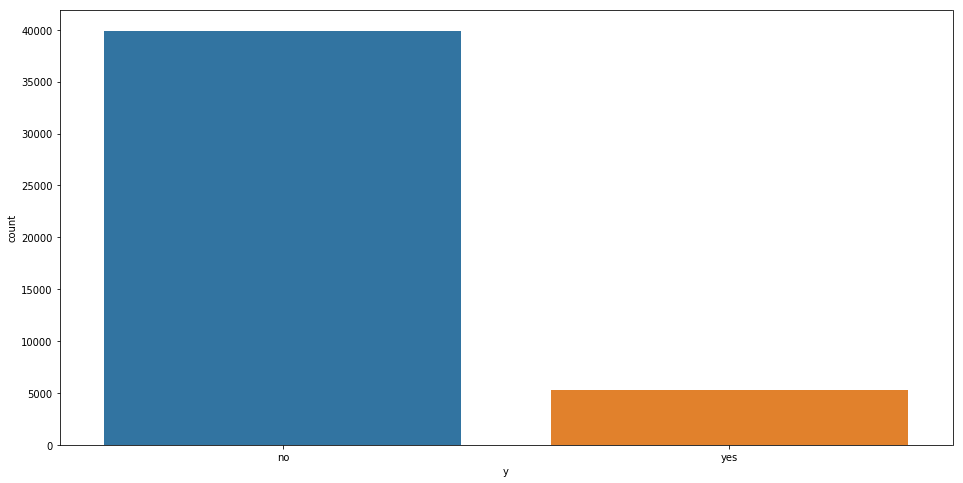
\includegraphics[width=1.0\textwidth]{images/fig1.png}
  \caption{Histograms of numeric variables.}
  \label{fig1}
\end{figure}

\begin{figure}
  \centering
    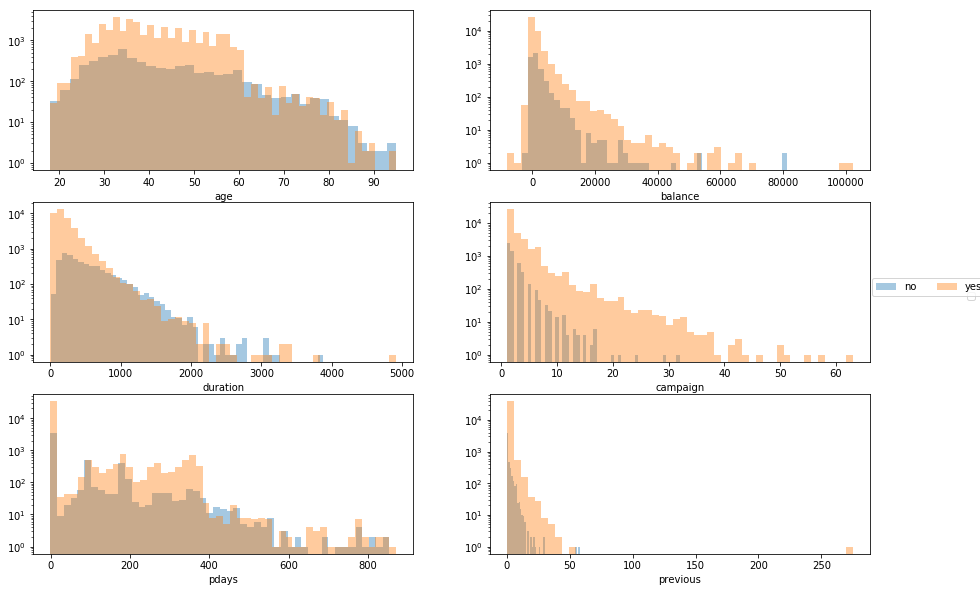
\includegraphics[width=1.0\textwidth]{images/fig2.png}
  \caption{Boxplots of numeric variables.}
  \label{fig2}
\end{figure}

\begin{figure}
  \centering
    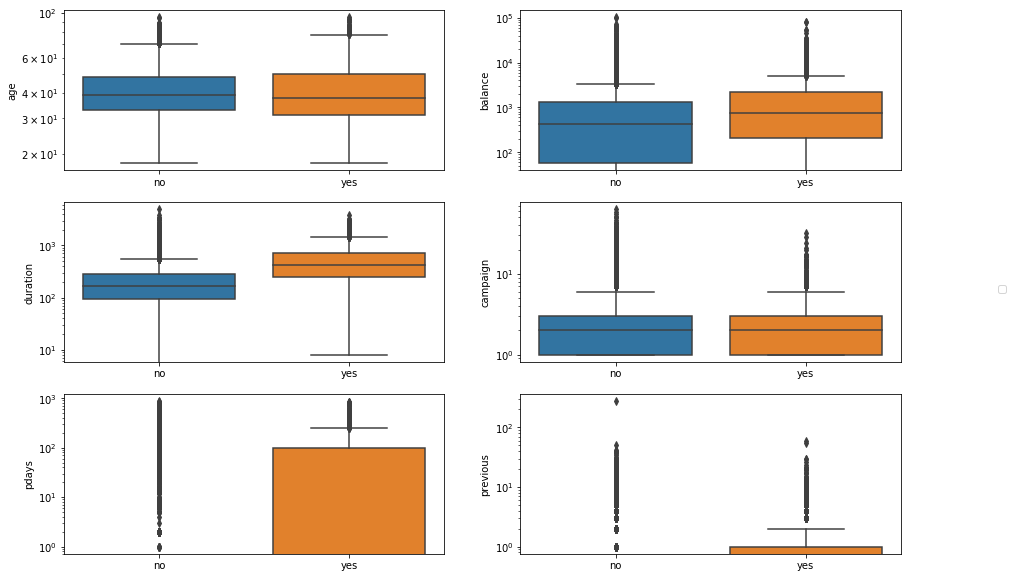
\includegraphics[width=0.7\textwidth]{images/fig3.png}
  \caption{Count plots of categorical variables.}
  \label{fig3}
\end{figure}

\begin{figure}
  \centering
    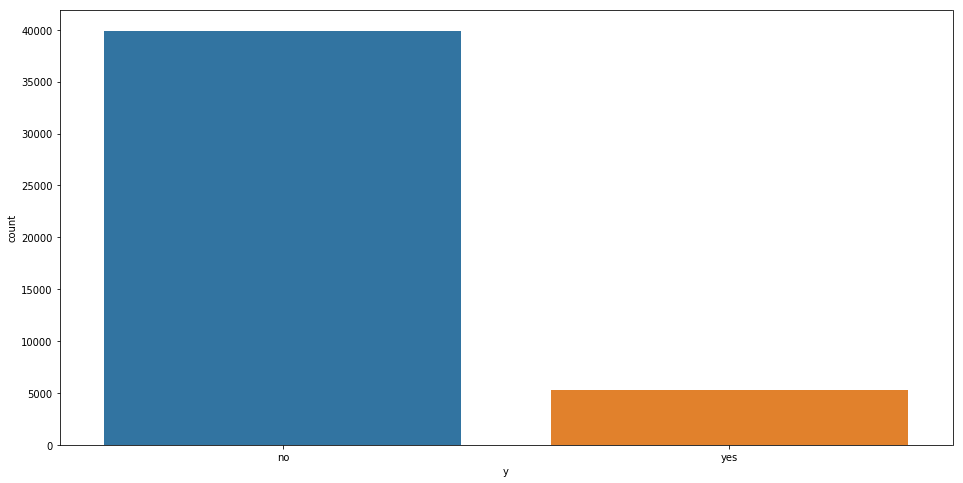
\includegraphics[width=0.5\textwidth]{images/fig4.png}
  \caption{Count plot of the response variable.}
  \label{fig4}
\end{figure}

\begin{figure}
  \centering
    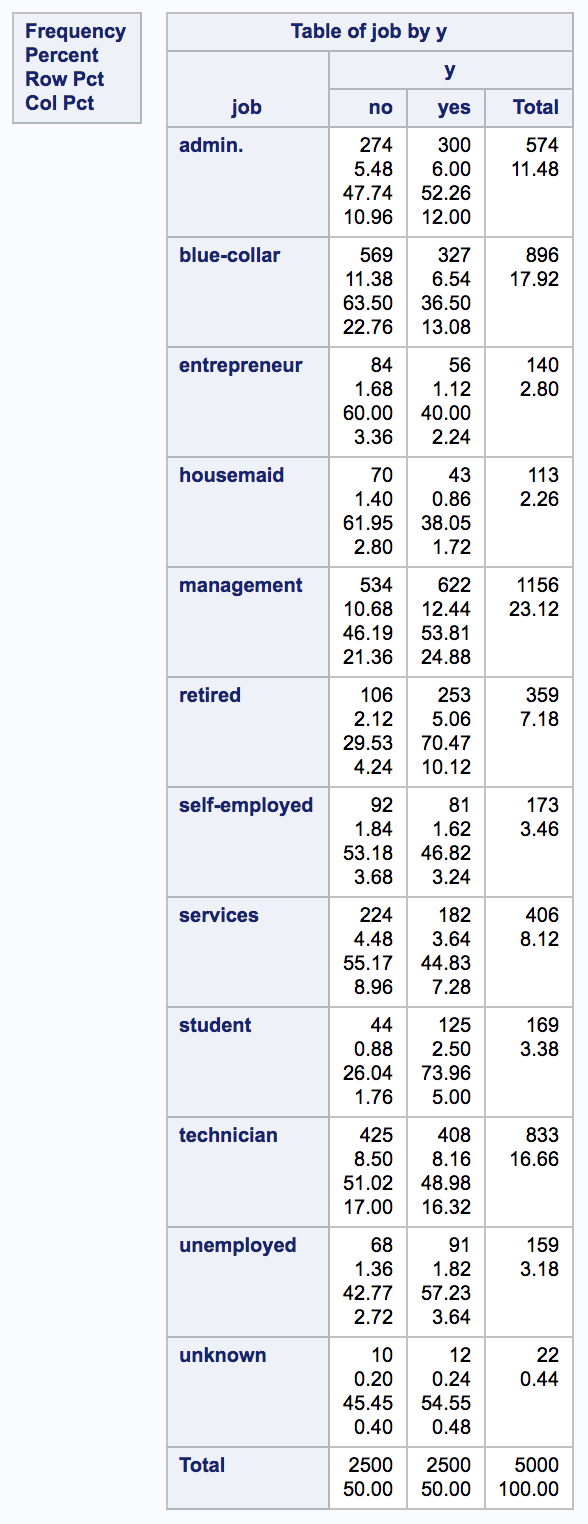
\includegraphics[width=0.5\textwidth]{images/fig5_job.png}
  \caption{Frequency table of job type by the response variable.}
  \label{fig5}
\end{figure}

\begin{figure}
  \centering
    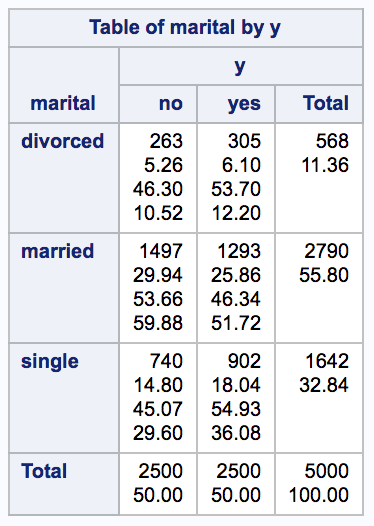
\includegraphics[width=0.5\textwidth]{images/fig6_marital.png}
  \caption{Frequency table of marital status by the response variable.}
  \label{fig6}
\end{figure}

\begin{figure}
  \centering
    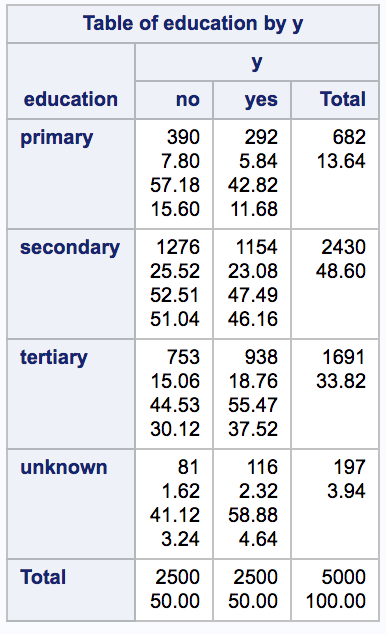
\includegraphics[width=0.5\textwidth]{images/fig7_educ.png}
  \caption{Frequency table of education level by the response variable.}
  \label{fig7}
\end{figure}

\begin{figure}
  \centering
    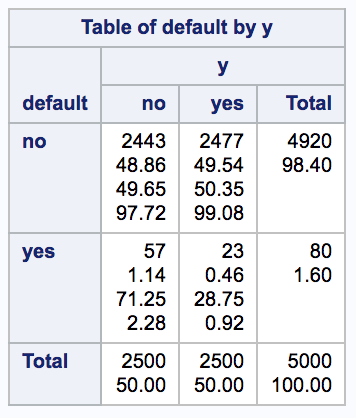
\includegraphics[width=0.5\textwidth]{images/fig8_default.png}
  \caption{Frequency table of default (has credit or not) by the response variable.}
  \label{fig8}
\end{figure}

\begin{figure}
  \centering
    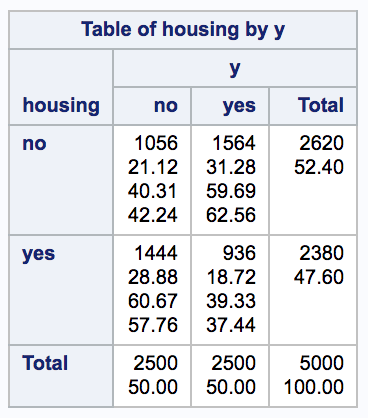
\includegraphics[width=0.5\textwidth]{images/fig9_housing.png}
  \caption{Frequency table of housing loan by the response variable.}
  \label{fig9}
\end{figure}

\begin{figure}
  \centering
    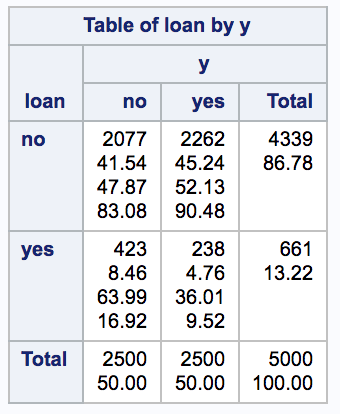
\includegraphics[width=0.5\textwidth]{images/fig10_loan.png}
  \caption{Frequency table of personal loan by the response variable.}
  \label{fig10}
\end{figure}

\begin{figure}
  \centering
    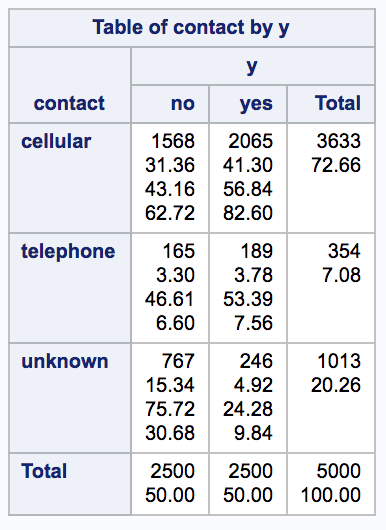
\includegraphics[width=0.5\textwidth]{images/fig11_contact.png}
  \caption{Frequency table of contact type by the response variable.}
  \label{fig11}
\end{figure}

\begin{figure}
  \centering
    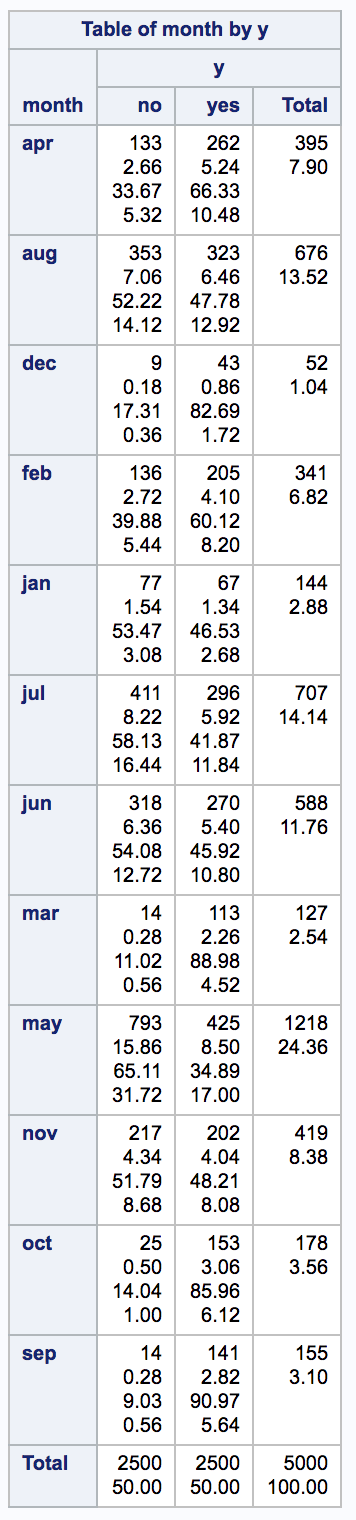
\includegraphics[width=0.5\textwidth]{images/fig12_month.png}
  \caption{Frequency table of last contact month by the response variable.}
  \label{fig12}
\end{figure}

\begin{figure}
  \centering
    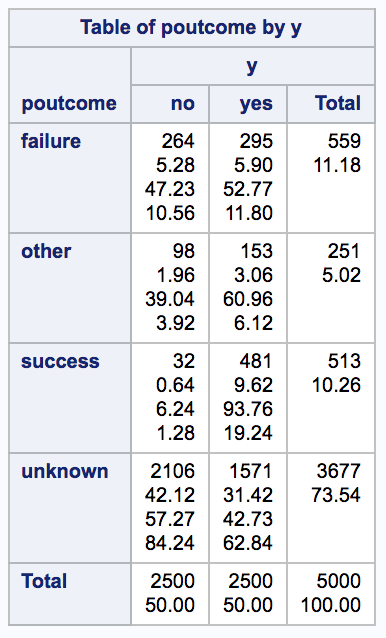
\includegraphics[width=0.5\textwidth]{images/fig13_poutcome.png}
  \caption{Frequency table of the outcome of the previous marketing campaign by the response variable.}
  \label{fig13}
\end{figure}

\begin{figure}
  \centering
    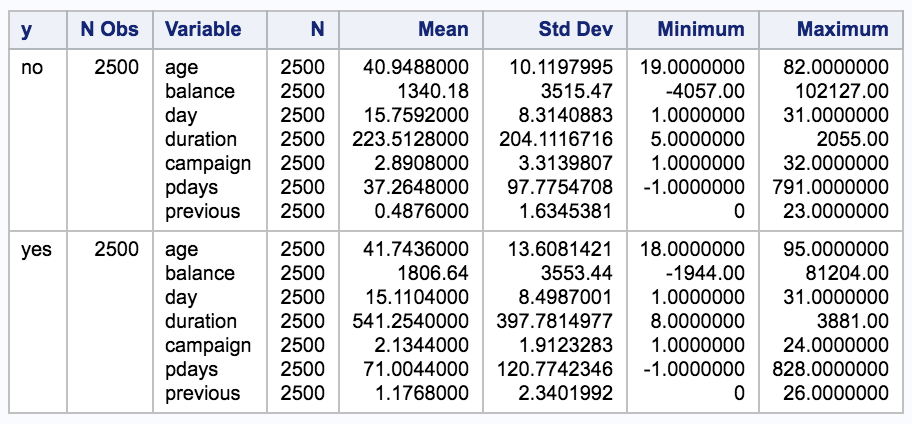
\includegraphics[width=0.8\textwidth]{images/fig14_summary.png}
  \caption{Summary statistics of the continuous variables by the response variable.}
  \label{fig14}
\end{figure}

\begin{figure}
  \centering
    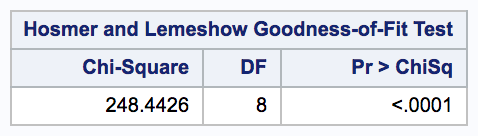
\includegraphics[width=0.5\textwidth]{images/fig15_GOF.png}
  \caption{Hosmer and Lemeshow Goodness-of-Fit Test Result.}
  \label{fig15}
\end{figure}

\begin{figure}
  \centering
    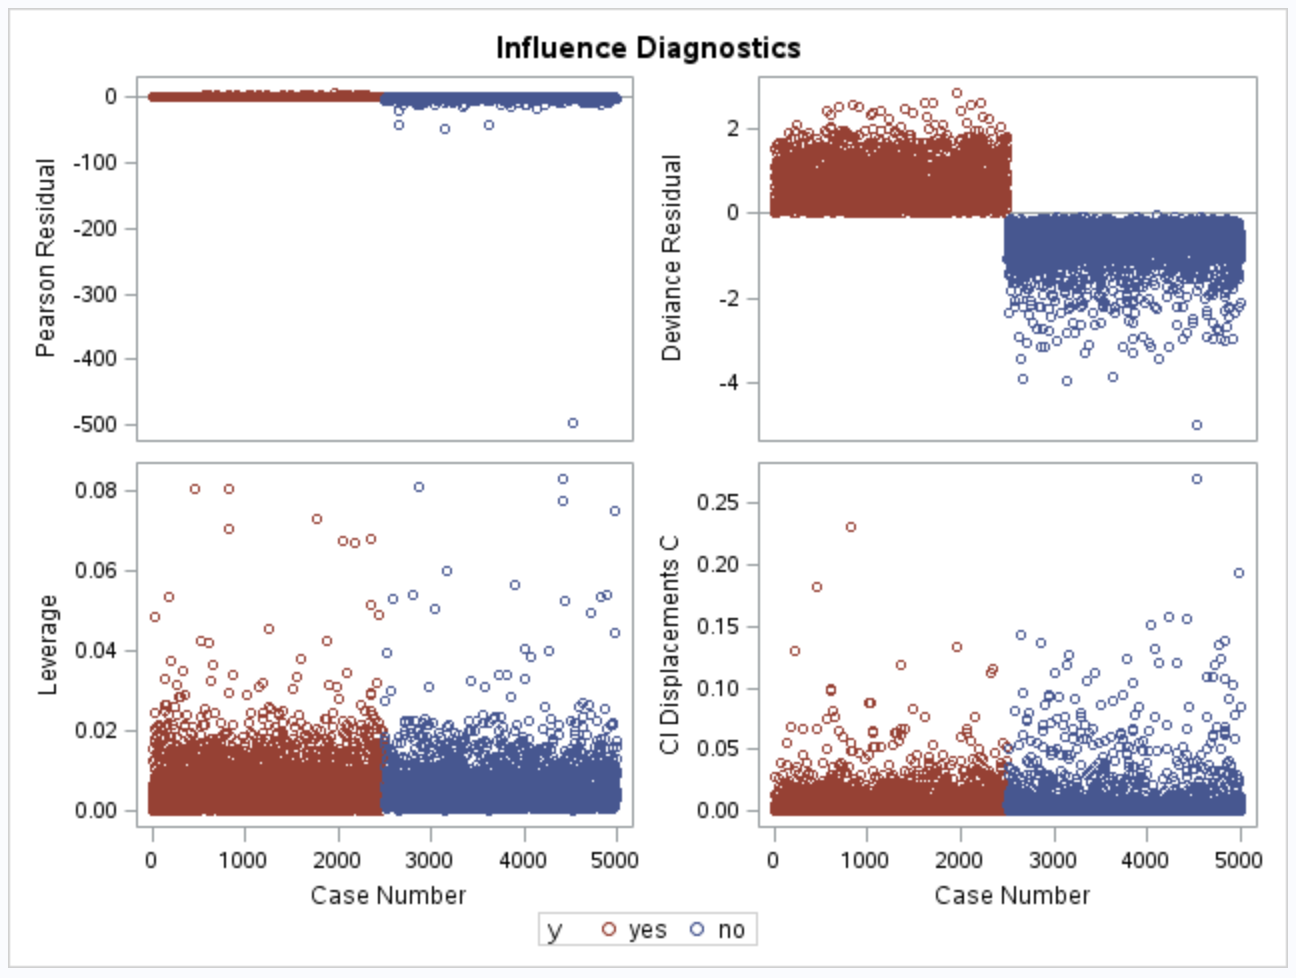
\includegraphics[width=0.4\textwidth]{images/fig16_residual_1.png}
    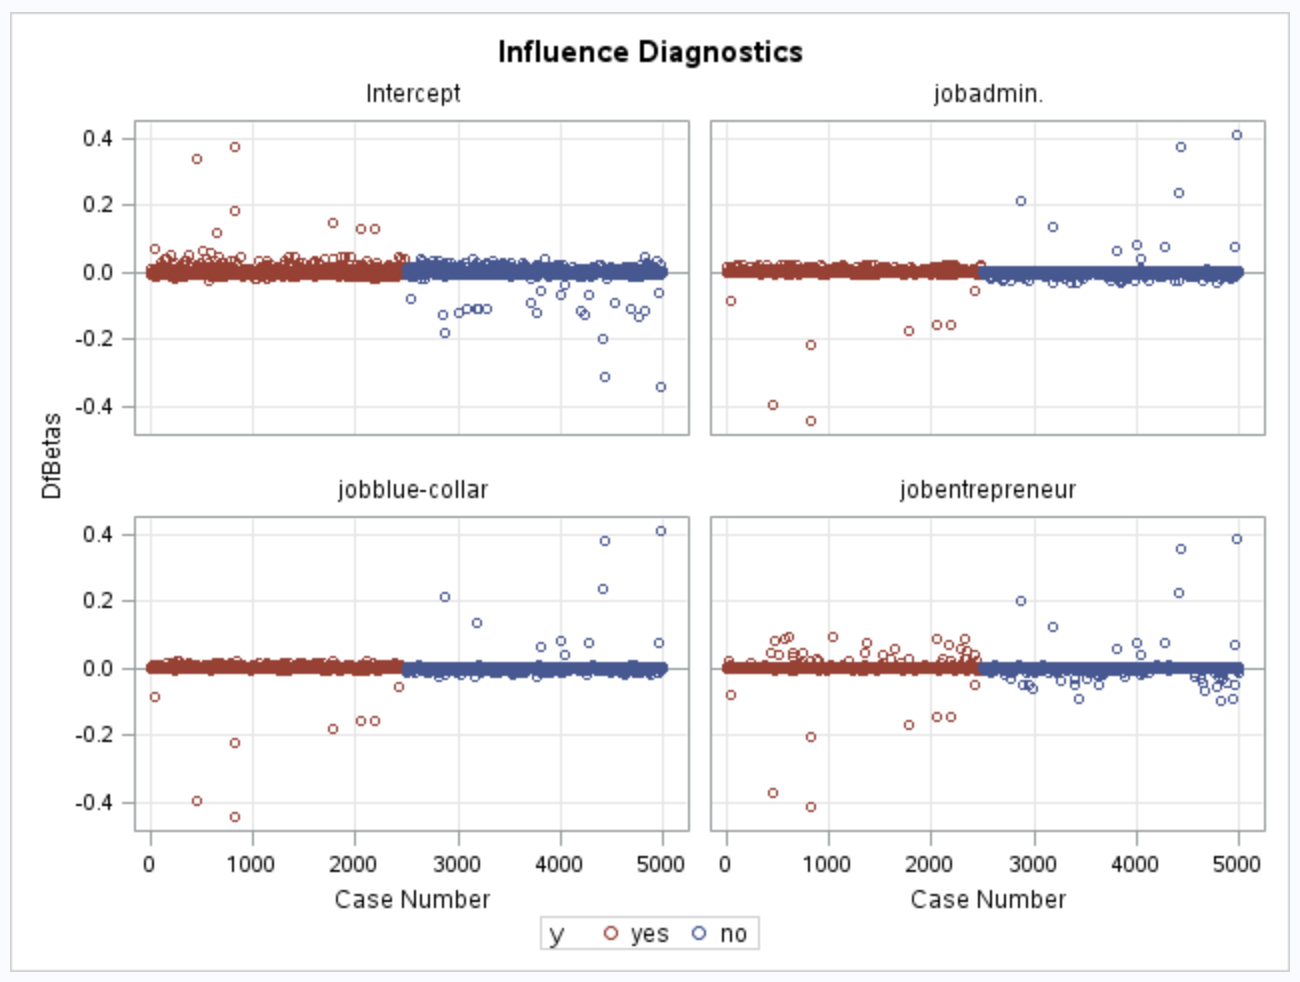
\includegraphics[width=0.4\textwidth]{images/fig16_residual_2.png}
    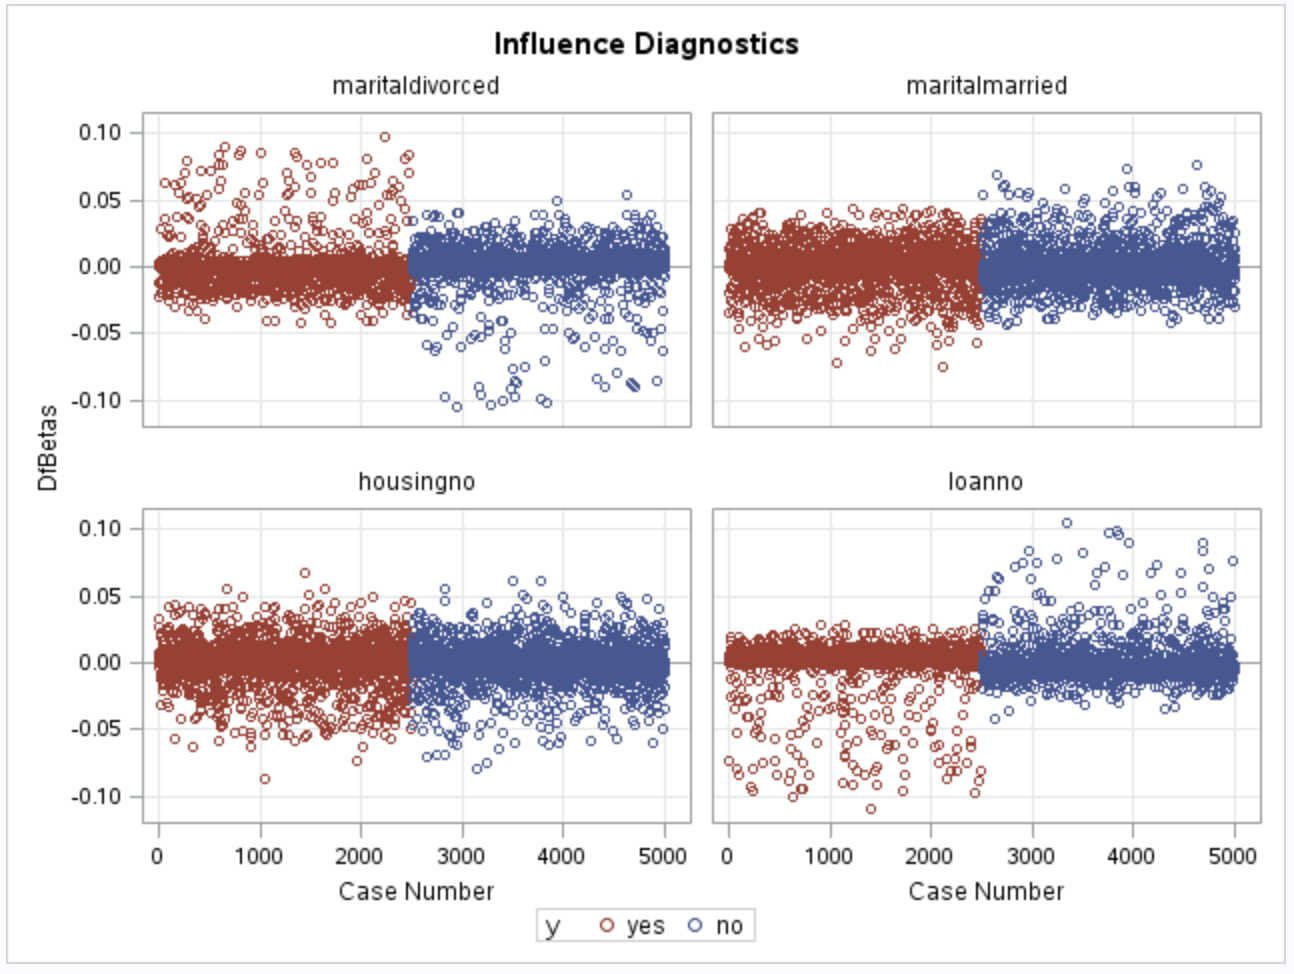
\includegraphics[width=0.4\textwidth]{images/fig16_residual_3.png}
    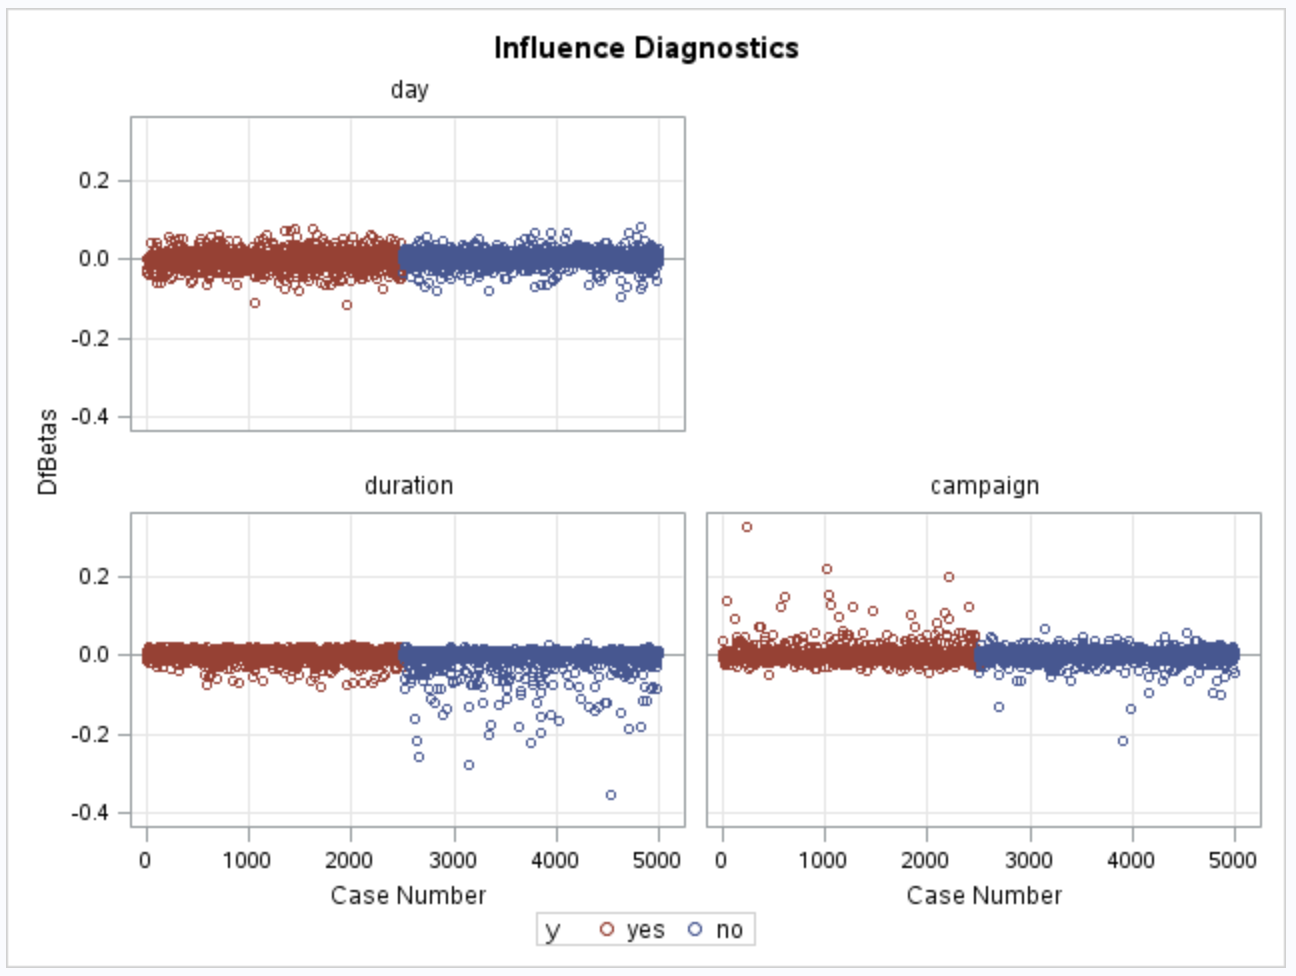
\includegraphics[width=0.4\textwidth]{images/fig16_residual_4.png}
  \caption{Residual and influential diagnostics plots.}
  \label{fig16}
\end{figure}

\begin{figure}
  \centering
    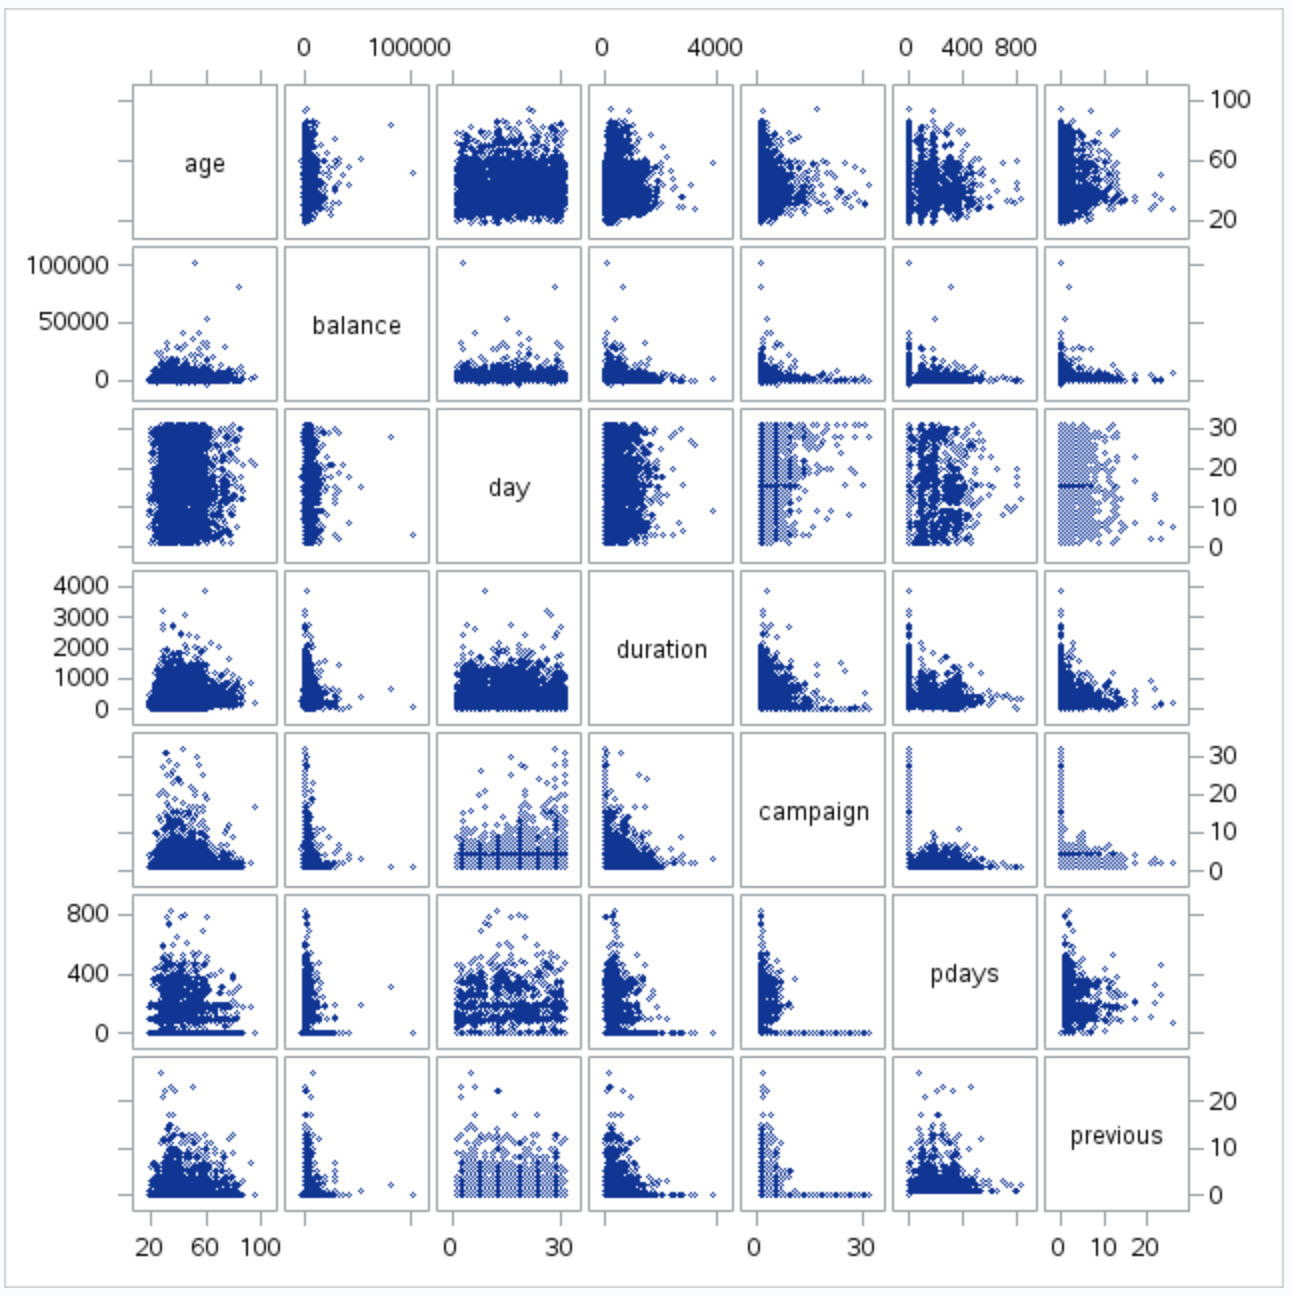
\includegraphics[width=0.6\textwidth]{images/fig17_scatter.png}
  \caption{Matrix scatterplot of the continuous explanatory variables.}
  \label{fig17}
\end{figure}

\begin{figure}
  \centering
    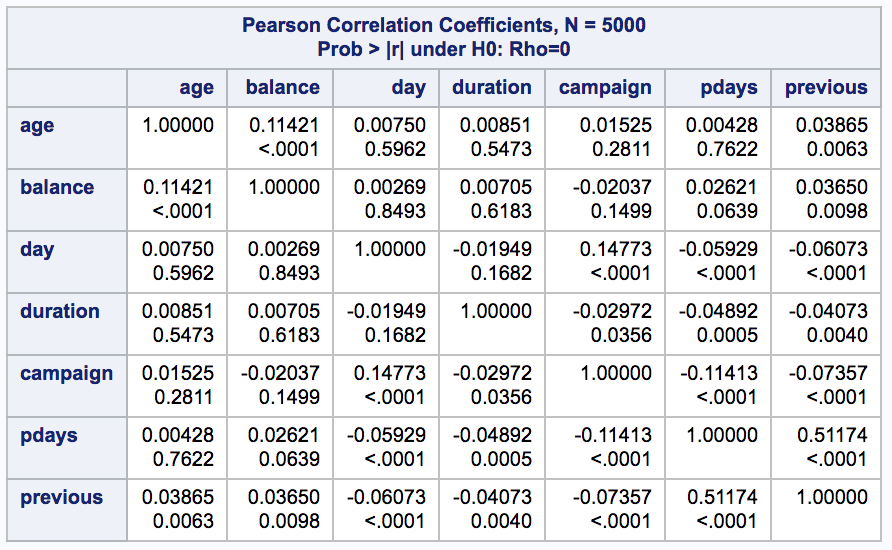
\includegraphics[width=0.8\textwidth]{images/fig18_corr.png}
  \caption{Correlation matrix of the continuous explanatory variables.}
  \label{fig18}
\end{figure}

\begin{figure}
  \centering
    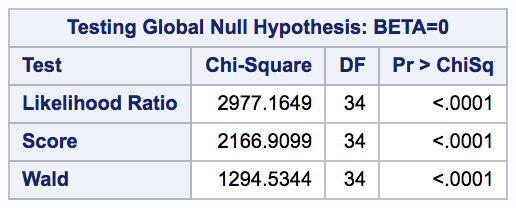
\includegraphics[width=0.5\textwidth]{images/fig19_overall_test.png}
  \caption{Overall test of Logistic Regression.}
  \label{fig19}
\end{figure}

\begin{figure}
  \centering
    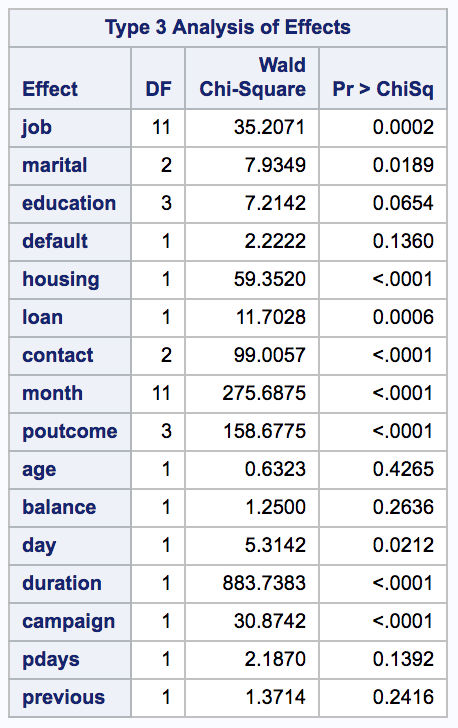
\includegraphics[width=0.5\textwidth]{images/fig20a_typeIII.png} 
    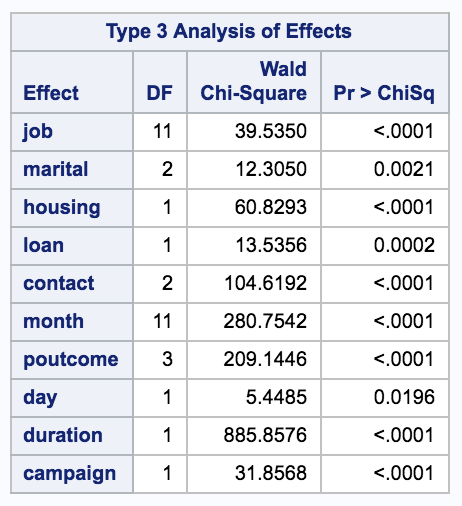
\includegraphics[width=0.5\textwidth]{images/fig20b_typeIII.png}
  \caption{Type 3 analysis of effects with all the predictors (left) and with only the predictors that are significant (right) using the balanced dataset.}
  \label{fig20}
\end{figure}

\begin{figure}
  \centering
    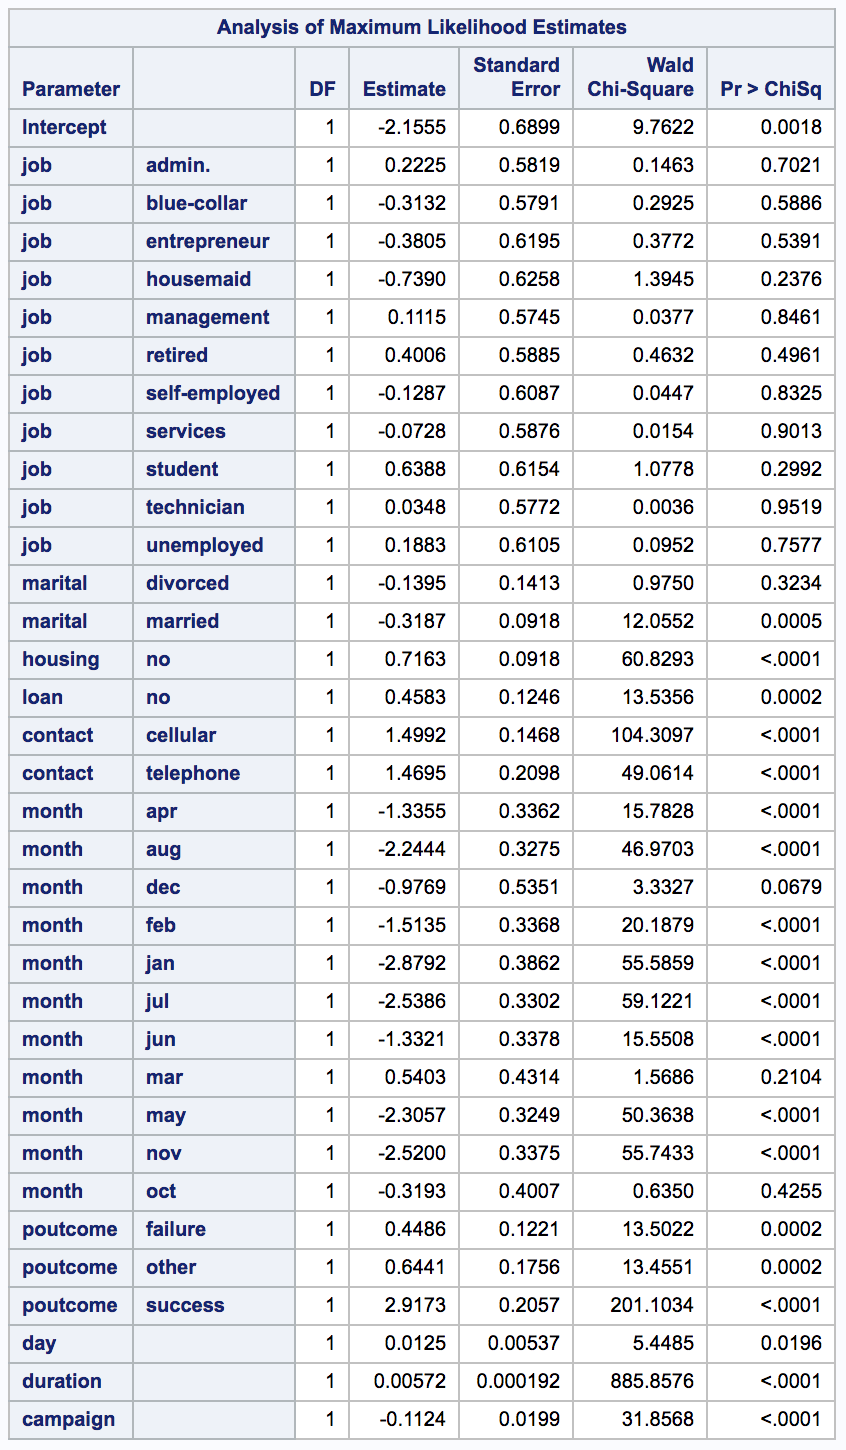
\includegraphics[width=0.8\textwidth]{images/fig21a_coefficients.png} 
  \caption{Tables of Coefficient estimates and Odds Ratio Estimates.}
  \label{fig21a}
\end{figure}

\begin{figure}
  \centering
    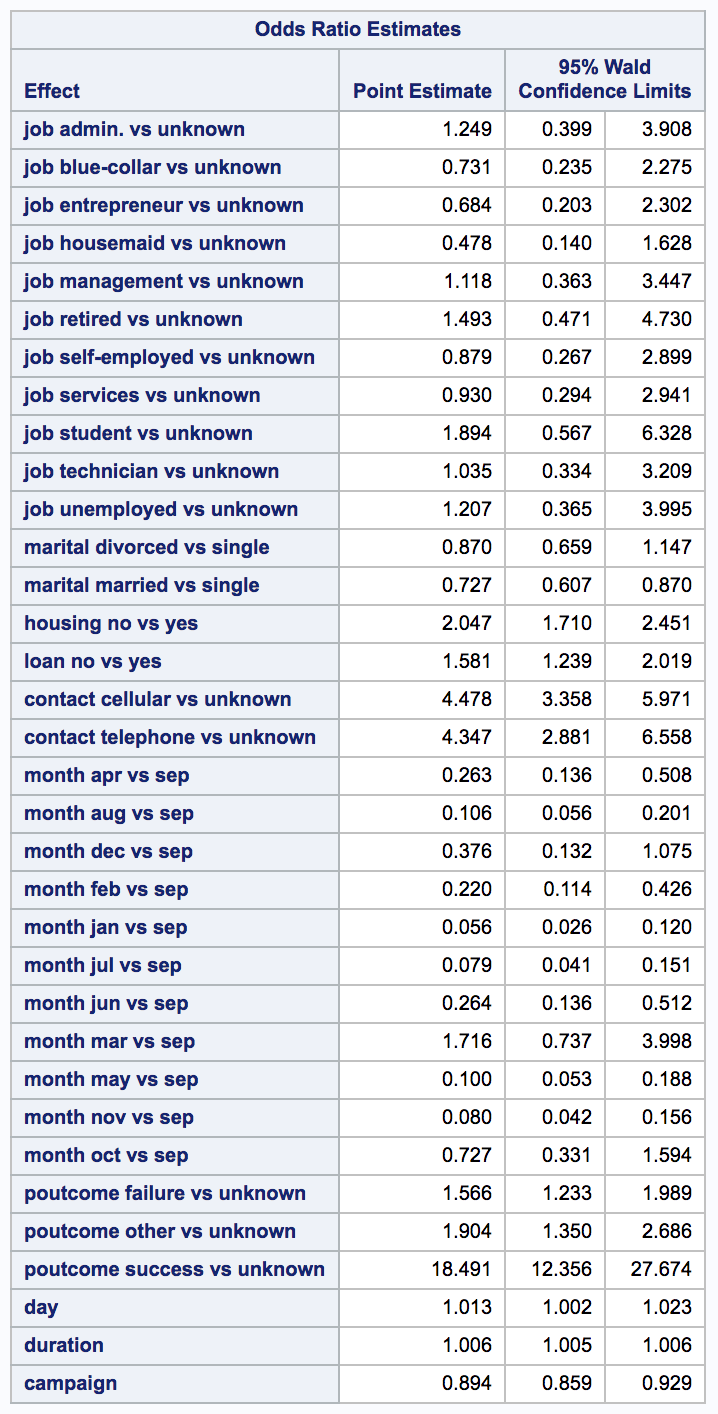
\includegraphics[width=0.8\textwidth]{images/fig21b_odds.png}
  \caption{Tables of Coefficient estimates and Odds Ratio Estimates.}
  \label{fig21b}
\end{figure}

\begin{figure}
  \centering
    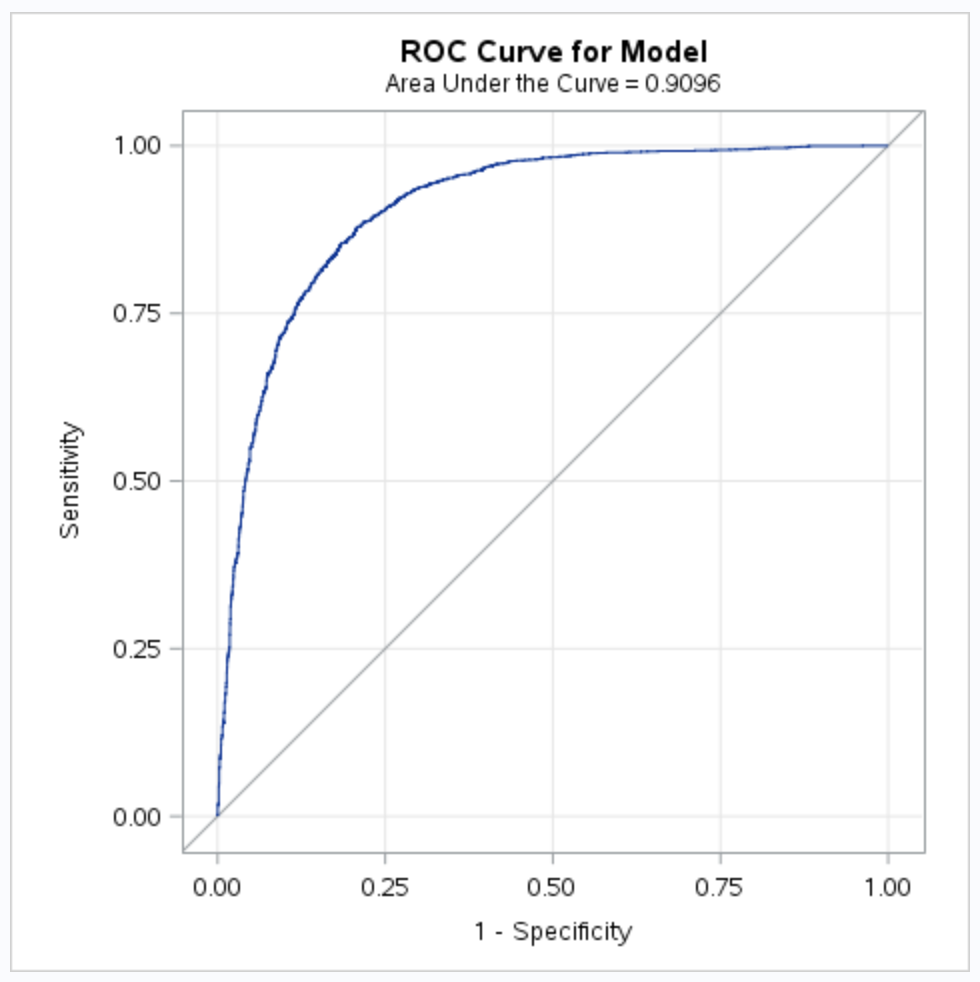
\includegraphics[width=0.5\textwidth]{images/fig22a_ROC.png} 
    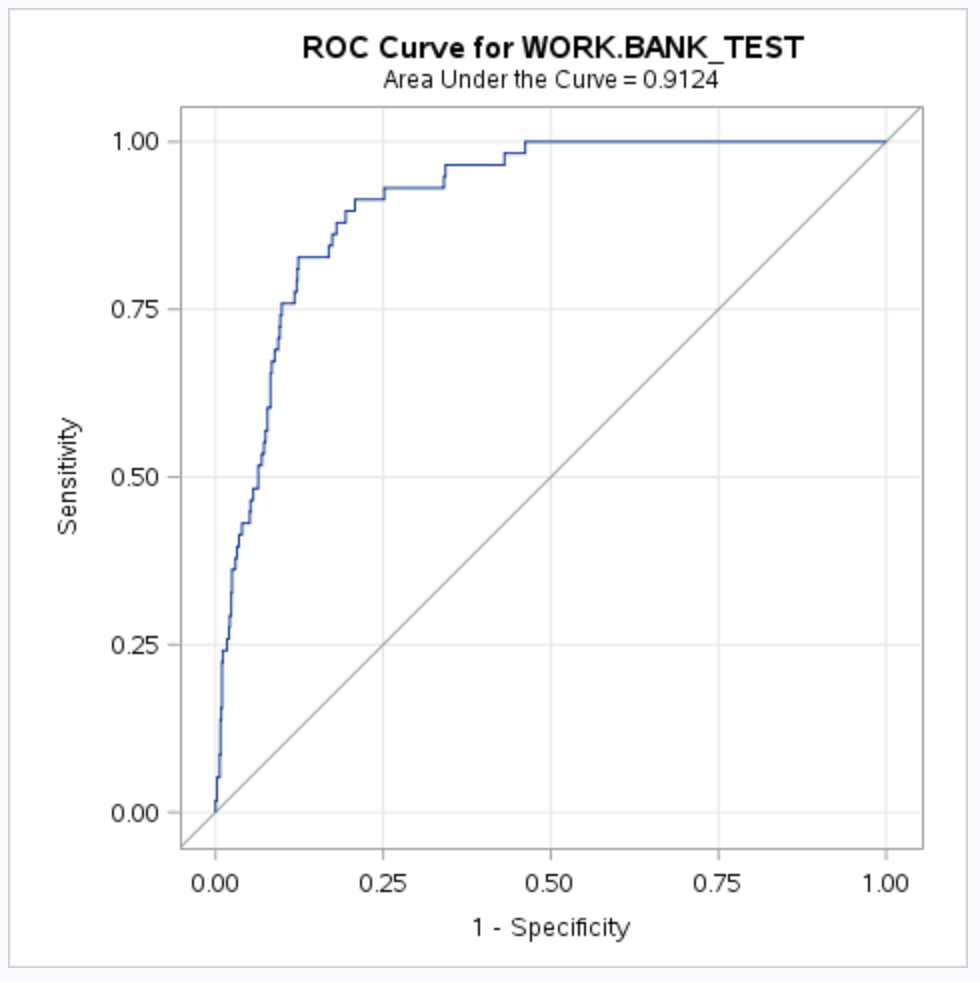
\includegraphics[width=0.5\textwidth]{images/fig22b_ROC.png}
  \caption{ROC curves for the balanced training dataset and the test dataset.}
  \label{fig22}
\end{figure}

\begin{figure}
  \centering
    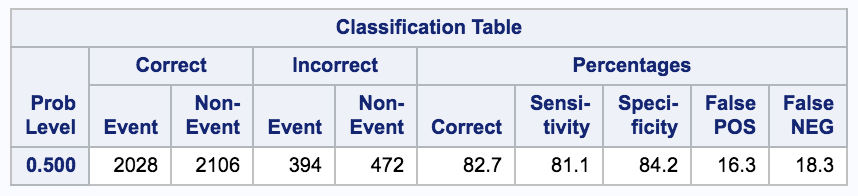
\includegraphics[width=0.5\textwidth]{images/fig23_ctable.png} 
  \caption{The classification table based on the balanced training dataset.}
  \label{fig23}
\end{figure}

\begin{figure}
  \centering
    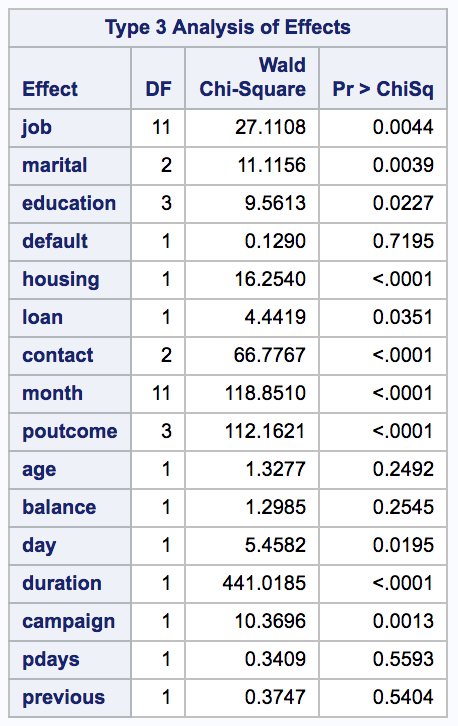
\includegraphics[width=0.5\textwidth]{images/fig24a_typeIII.png} 
    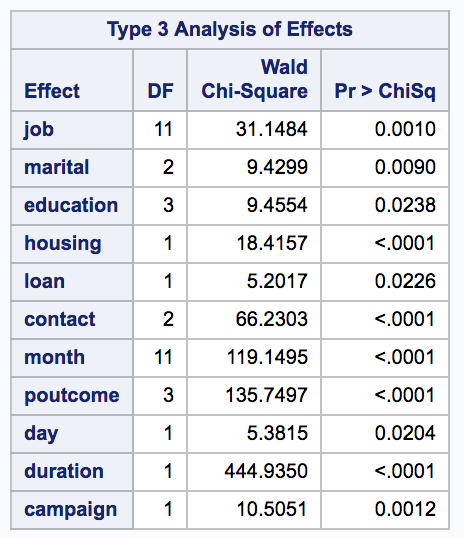
\includegraphics[width=0.5\textwidth]{images/fig24b_typeIII.png}
  \caption{Type 3 analysis of effects with all the predictors (left) and with only the predictors that are significant (right) using the unbalanced training dataset.}
  \label{fig24}
\end{figure}

\begin{figure}
  \centering
    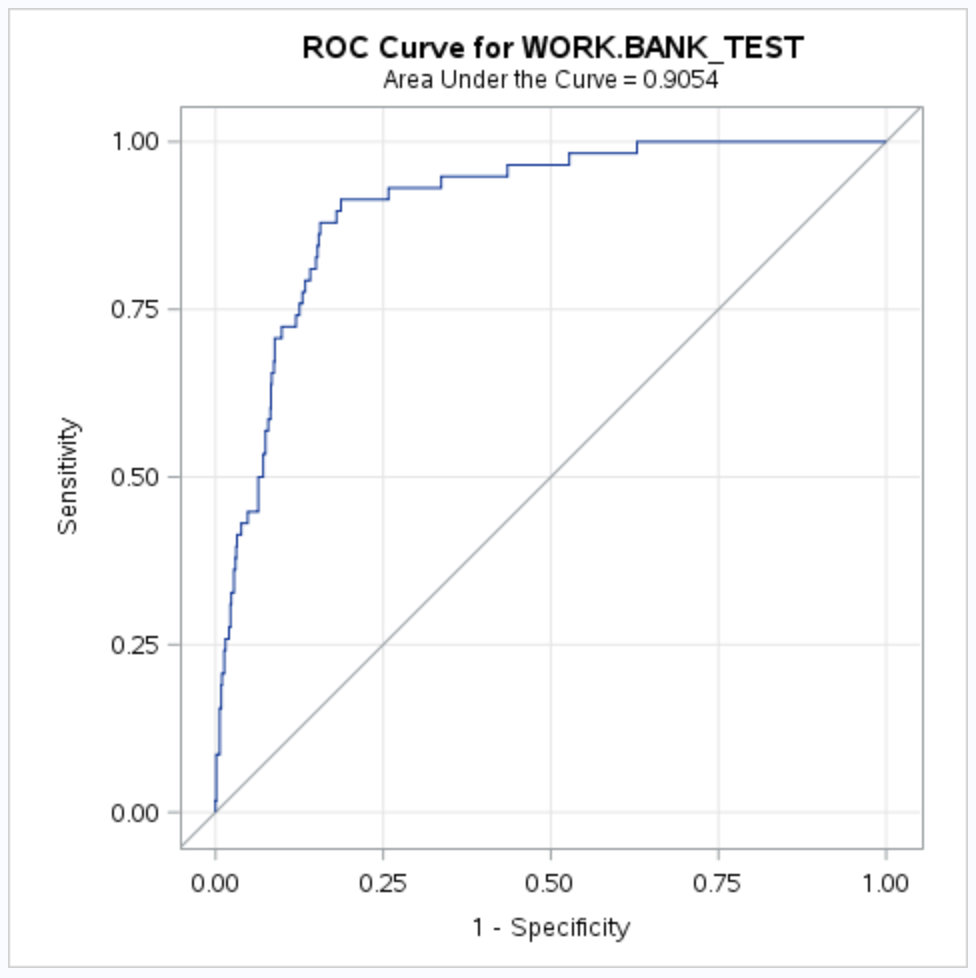
\includegraphics[width=0.5\textwidth]{images/fig25a_ROC.png} 
    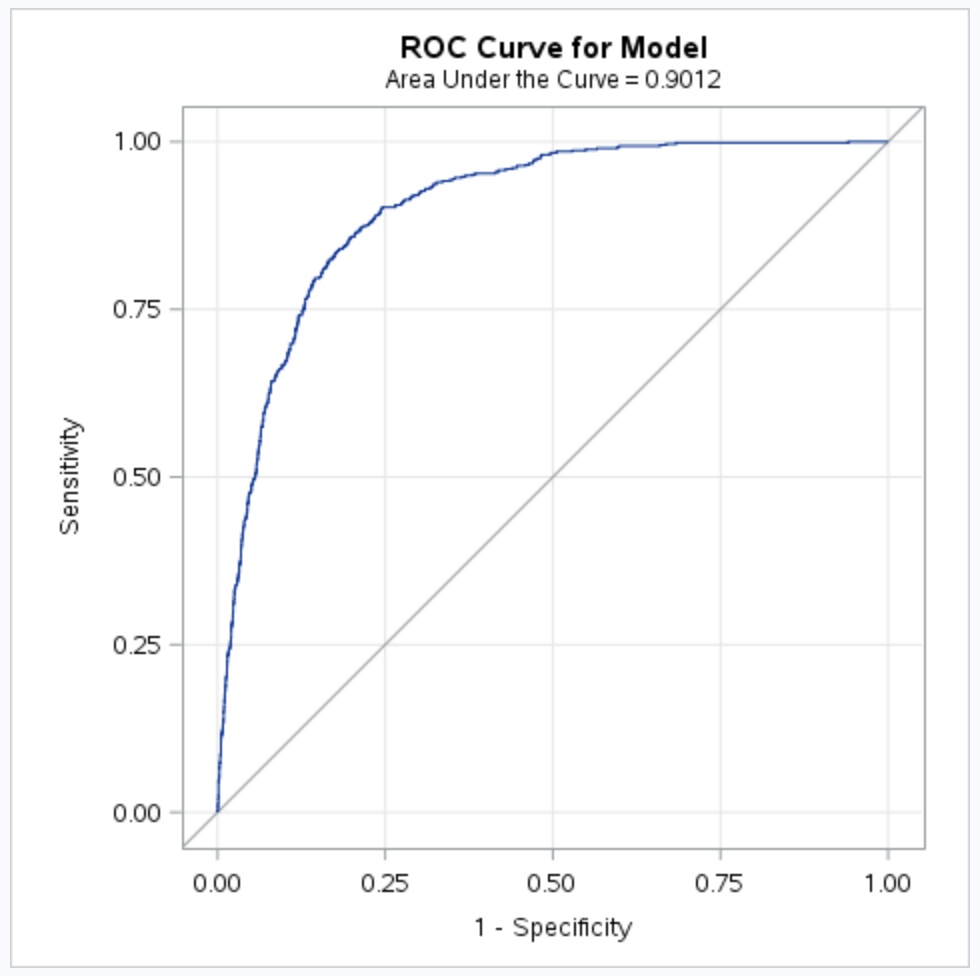
\includegraphics[width=0.5\textwidth]{images/fig25b_ROC.png}
  \caption{ROC curves for the unbalanced training dataset and the test dataset.}
  \label{fig25}
\end{figure}

\begin{figure}
  \centering
    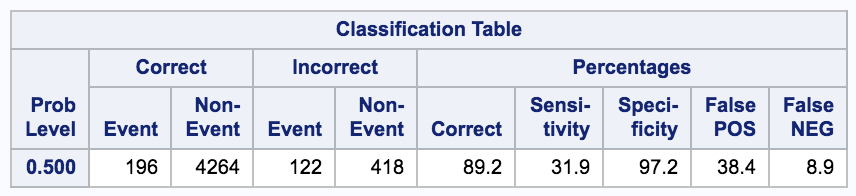
\includegraphics[width=0.5\textwidth]{images/fig26_ctable.png} 
  \caption{The classification table based on the unbalanced training dataset.}
  \label{fig26}
\end{figure}


\end{document}
